%-- steuerung der evolution

\section{Steuerung der Evolution}

In diesem Kapitel werden die wesentlichen Evolutionsstrategien sowie deren Handlungsabfolge mithilfe von Pseudocode-Abschnitten näher beschrieben.

\subsection{$(1+1)$-ES}

Die $(1+1)$-Evolutionsstrategie gilt als einfachste Form der ES. Bereits damit hat Rechenberg 1964 die optimale Einstellung von Gelenkwinkeln einer Gelenkplatte berechnen lassen.

Es handelt sich um eine zweigliedrige Strategie, bei dem es in jeder Evolutionsiteration genau ein Ur-Individuum bzw. Elternindividuum gibt, welches der Erzeugung von genau einem nachkommenden Individuum (Kindindividuum) dient. Dabei wird der Ausgangsvektor analog zum biologischen Prozess der DNS-Selbstverdopplung dupliziert. Das zweite, bislang wertgleiche, Individuum wird anschließend zufällig, allerdings nicht willkürlich, modifiziert. Meist wird ein kleiner reeller Wert auf jeden Vektorparameter addiert.

Die beiden, nun unterschiedlichen, Individuen werden nach dem Prinzip \enquote{survival of the fittest} bewertet.
Anhand des Outputs einer Qualitätsfunktion wird verglichen, welcher der beiden Individuen das angemessenere ist und anschließend zur Fortführung der Evolution selektiert werden soll.
Umgangssprachlich spricht man von einem \enquote{Sterben der Schwachen} und einem \enquote{Überleben der Starken}.
Bei gleicher Qualitätsbewertung wird ein Individuum zufällig selektiert.
Als Zeitmaß für die Evolutionsiteration dient die \enquote{Generation}, wobei die Generation $G_0$ die Ausgangsgeneration mit einem Ausgangsindividuum bildet. Die Selektion aus dessen Elterindividuum sowie dessen Nachkomme bildet die Generation $G_1$ und so weiter.

Aus diesem Vorgehen bedeutet die Namensgebung "$(1+1)$-ES": Ein Elternindividuum wird zusammen mit einem nachkommenden Individuum für die Selektion betrachtet.

In diesem Fall wird das Erbgut ausschließlich über die Mutation verändert. Es gibt keine sexuelle Rekombination des Erbgutes.

Es handelt sich zwar um eine grundlegende und kompakte Form der Abbildung von Evolutionsmechanismen, jedoch können auch hierbei in Kombination mit der adaptiven Schrittweitenregelung zur Mutation der Nachkommen (\textit{siehe Kapitel \ref{sec:mutation}}) sinnvolle Anwendungen entstehen.

Abbildung \ref{fig:1_und_1_es} veranschaulicht den Ablauf anhand der Rechenberg'schen Grafik-Notation. Da bereits bei dieser einfachen Evolutionsstrategie eine recht flächendeckende Veranschaulichung benötigt wird, welche mit steigender Komplexität wesentlich schwerer zu überblicken ist, wurde auf eine Veranschaulichung der weiteren Evolutionsstrategien verzichtet. 

\begin{figure}[H]
\centering
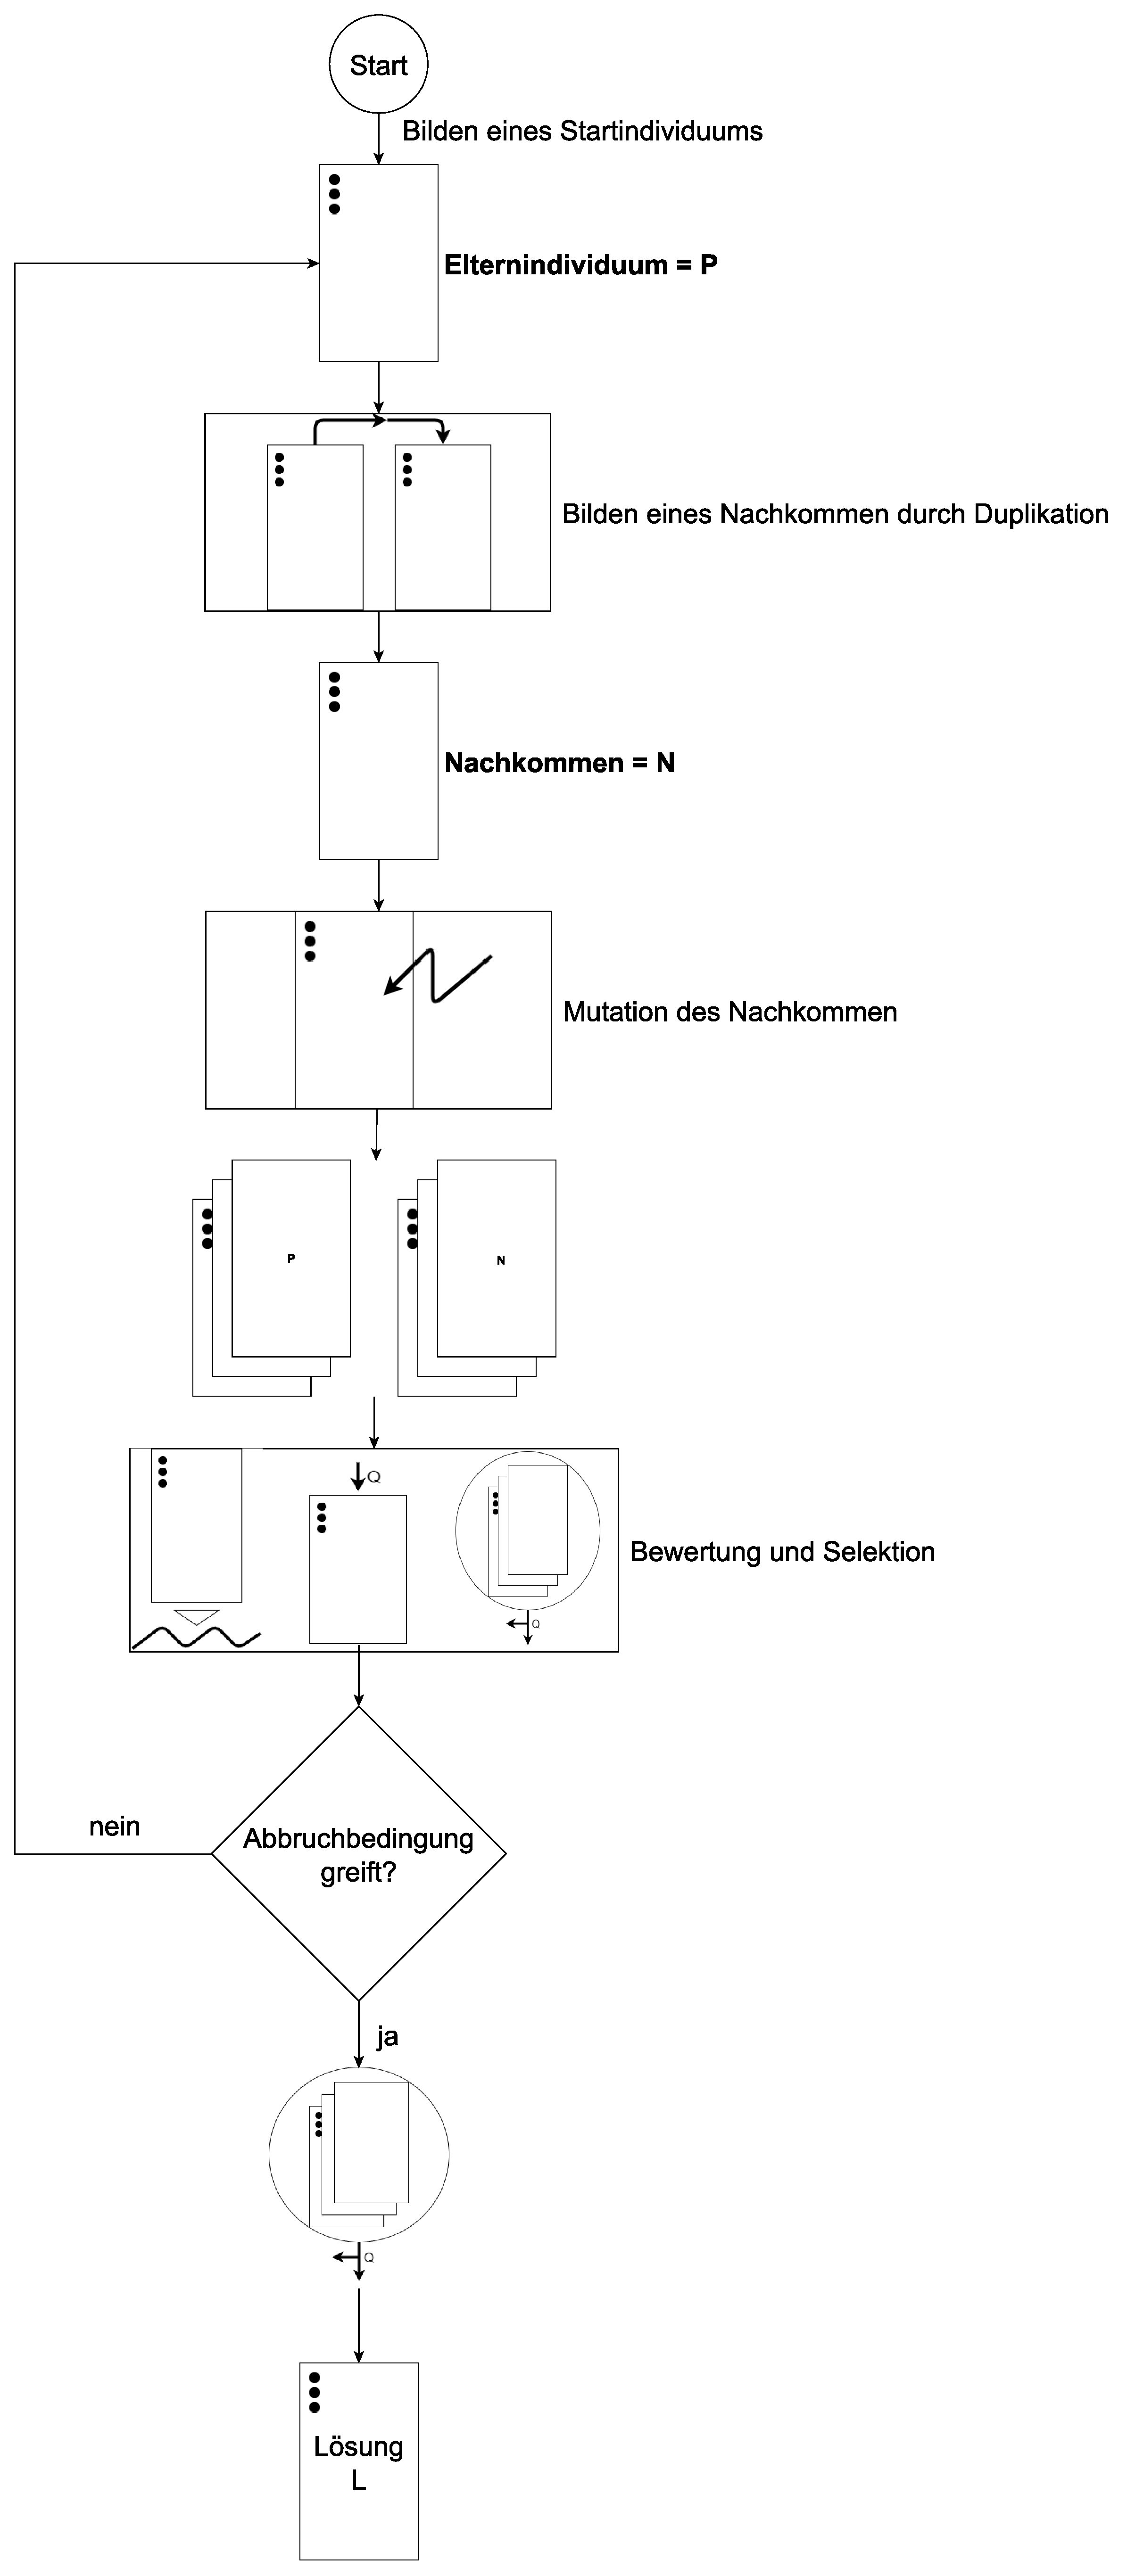
\includegraphics[width=0.4\textwidth]{img/1_und_1_es.pdf}
\caption{$(1+1)$-ES}
\label{fig:1_und_1_es}
\end{figure}

Folgender Pseudocode-Abschnitt \ref{lst:1_und_1_es} verdeutlicht die grundlegende Vorgehensweise. Während die grüne Zeilenmarkierung den Beginn der wesentlichen Evolutionsstrategie hervorhebt, hebt eine blaue Markierung die nun relevanten Unterschiede im Vergleich zur jeweils vorigen Evolutionsstrategie hervor.

\begin{lstlisting}[caption={$(1+1)$-Evolutionsstrategie}, firstnumber=1, captionpos=b, label=lst:1_und_1_es]
<@\colorcodeline{algorithm baue\_individuum(n)}@>
	individuum <- []	
	for _ <- 1,...,n
		individuum <- individuum + zufälliges $x \in \mathbb{R}$
	return individuum
	
<@\colorcodeline{algorithm qualitaet(individuum | population)}@>
	// problemspezifische Qualitätsfunktion

	
<@\colorcodeline{algorithm duplikation(individuum[1,...,n])}@>
	klon <- []
	for i <- 1,...,n
		klon <- klon + individuum[i]
	return klon
	
<@\colorcodeline{algorithm selektion(individuen[1,...,m], $\mu$, qualitaetsfunktion)}@>
	sortierteIndividuen <- sortiereAbsteigend(individuen, qualitaetsfunktion)
	besteIndividuen <- []
	for i <- 1,...,$\mu$
		besteIndividuen <- besteIndividuen + sortierteIndividuen[i]
	return besteIndividuen

<@\colorcodealgorithm{algorithm $(1+1)$-ES()}@>
	iterationsLimit <- x $\in \mathbb{N}$
	generationszaehler <- 0
	wunschqualitaet <- y $\in \mathbb{R}$
	individuengroesse <- n $\in \mathbb{N}$
	<@\colorcodeline{individuum <- baue\_individuum(individuengroesse)}@>
	while qualitaet(individuum) < wunschqualitaet and generationszaehler < iterationslimit
		generationszaehler <- generationszaehler + 1
		elter <- individuum
		<@\colorcodeline{kind <- duplikation(elter)}@>
		kind <- mutation(kind)
		individuum <- selektion([elter, kind], 1, qualitaet)
	loesung <- individuum
	return loesung
\end{lstlisting}

\subsection{$(\mu + \lambda)$-ES}

Mit der $(\mu + \lambda)$-Evolutionsstrategie wird die vorige $(1+1)$-ES in einer allgemeineren Form übertragen.
Dabei gilt:

\begin{equation}
1 \le |Eltern| \le |Nachkommen| \Leftrightarrow 1 \le \mu \le \lambda
\end{equation}
\myequations{Beziehung zwischen Eltern und Kinder}

Es müssen aus den $\mu$ Eltern also $\lambda$ Nachkommen erzeugt werden, wobei es mindestens genau so viele Nachkommen wie Eltern geben muss.
Alle Individuen werden gemeinsam für eine Selektion der besten Individuen betrachtet, sowohl die Eltern als auch die Kinder.
Somit können einige Elternindividuen über mehrere Generationen hinweg bestehen, sofern sie sich einem im Vergleich hohen Qualitätswert zuordnen lassen.

Das \enquote{+} der $(\mu + \lambda)$-Notation lässt sich somit als Vereinigung sowohl der Eltern als auch der Nachkommen lesen, die abschließend gemeinsam selektiert werden.

Werden mehrere Nachkommen erzeugt als es Eltern gibt, also:

\begin{equation}
|Nachkommen| > |Eltern| \Leftrightarrow \lambda > \mu
\end{equation}
\myequations{Bedingung für die Mehrfachselektion von Eltern}

dann müssen einige Eltern mehrfach zur Erzeugung eines Nachkommens ausgewählt werden.
Von allen Individuen werden anschließend die $|Eltern| = \mu$ besten als Basis für die nächste Generation ausgewählt. Die Größe der Elternpopulation bleibt somit immer konstant. Da die Eltern \textbf{und} die Nachkommen bewertet werden und zur Selektion bereitstehen, nimmt die Qualität des besten Individuums der nächsten Population im Vergleich zur vorigen niemals ab.

Algorithmisch sind die Anzahlen der Nachkommen und der Eltern folglich nun frei wählbar, wobei die Anzahl der zu erzeugenden Nachkommen anhand der erläuterten Bedingung mindestens so groß wie die Anzahl der Elternindividuen sein muss. Dies wird in Pseudocode \ref{lst:mu_und_lambda_es} dargestellt.

\begin{lstlisting}[caption={$(\mu + \lambda)$-Evolutionsstrategie}, firstnumber=1, captionpos=b, label=lst:mu_und_lambda_es]
<@\colorcodeline{algorithm baue\_population($\mu$, n)}@>
	population <- []
	for i <- 1,...,$\mu$
		individuum <- baue_individuum(n)
		population <- population + individuum
	return population
	
<@\colorcodeline{algorithm elternSelektion(population[1,...,$\mu$], $\lambda$)}@>
	individuen <- []
	for _ <- 1,...,$\lambda$
		idx <- zufälliges x $\in {1,...,\mu}$
		individuum <- population[idx]
		individuen <- individuen + individuum
	return individuen
	

<@\colorcodeline{algorithm duplikation(individuen[1,...,$\mu$], n)}@>
	klone <- []
	for i <- 1,...,$\mu$
		klon <- []
		for j <- 1...n
			klon <- klon + individuen[i][j]
		klone <- klone + klon
	return klon
	
<@\colorcodeline{algorithm bestenSelektion(population[1,...,$\mu$])}@>
	beste_loesung <- []
	for i <- 1,...,$\mu$
		individuum <- population[i]
		if qualitaet(individuum) > qualitaet(beste_loesung)
			beste_loesung <- individuum
	return beste_loesung
	

<@\colorcodealgorithm{algorithm $(\mu + \lambda)$-ES()}@>
	iterationsLimit <- x $\in \mathbb{N}$
	generationszaehler <- 0
	anzahl_eltern <- $\mu \ge 1$
	anzahl_kinder <- $\lambda \ge$ anzahl_eltern
	wunschqualitaet <- y $\in \mathbb{R}$
	individuengroesse <- n $\in \mathbb{N}$
	<@\colorcodeline{population <- baue\_population($\mu$, individuengroesse)}@>
	while qualitaet(population) < wunschqualitaet and generationszaehler < iterationslimit
		generationszaehler <- generationszaehler + 1
		<@\colorcodeline{eltern <- elternSelektion(population, anzahl\_kinder)}@>
		<@\colorcodeline{kinder <- duplikation(eltern, individuengroesse)}@>
		kinder <- mutation(kinder)
		<@\colorcodeline{population <- selektion(eltern + kinder, $\mu$, qualitaet)}@>
	loesung <- bestenSelektion(population)
	return loesung
\end{lstlisting}

\subsection{$(\mu, \lambda)$-ES}

Als weitere Evolutionsstrategie gibt es die Komma-Notation, welche von Schwefel in seiner Dissertation 1975 eingeführt wurde. Bei $(\mu + \lambda)$-ES kann das beste Individuum nicht vergessen gehen, da in jeder Iteration alle Individuen bei der Selektion berücksichtigt werden. Auf den ersten Blick klingt dies nach einem wünschenswerten Effekt, jedoch können negative Auswirkungen die Folge sein, wenn es sich dabei um ein lokales Optimum laut der Qualitätsfunktion handelt.
Das globale Optimum und somit die optimale Lösung des Problems wird daraufhin häufig nicht mehr gefunden.

Schwefels $(\mu, \lambda)$-ES nutzt einen veränderten Selektionsmechanismus:
Die Elternindividuen werden bei der abschließenden Selektion nicht mehr berücksichtigt und somit vergessen. Es werden lediglich $|Eltern| = \mu$ der $|Nachkommen| = \lambda$ Nachkommen für die nächste Generation ausgewählt.

Insofern handelt es sich um ein naturgetreues Modell der Evolution. Kein Individuum ist mehr unsterblich. Allerdings sterben sie direkt nach einer Generation. Aufgrund dessen sind allerdings auch Rückschritte in der Evolution möglich.

Generell werden geringfügige normalverteilte Mutationen bevorzugt, um nur leichte Veränderungen der Nachkommen hervorzurufen.

\begin{lstlisting}[caption={$(\mu, \lambda)$-Evolutionsstrategie}\label{lst:mu_nur_lambda_es}, firstnumber=1, captionpos=b, label=code:mu_nur_lambda_es]
<@\colorcodealgorithm{algorithm $(\mu , \lambda)$-ES()}@>
	iterationsLimit <- x $\in \mathbb{N}$
	generationszaehler <- 0
	anzahl_eltern <- $\mu \ge 1$
	anzahl_kinder <- $\lambda \ge$ anzahl_eltern
	wunschqualitaet <- y $\in \mathbb{R}$
	individuengroesse <- n $\in \mathbb{N}$
	population <- baue_population($\mu$, individuengroesse)
	while qualitaet(population) < wunschqualitaet and generationszaehler < iterationslimit
		generationszaehler <- generationszaehler + 1
		eltern <- elternSelektion(population, anzahl_kinder)
		kinder <- duplikation(eltern, individuengroesse)
		kinder <- mutation(kinder)
		<@\colorcodeline{population <- selektion(kinder, $\mu$, qualitaet)}@>
	loesung <- bestenSelektion(population)
\end{lstlisting}

\subsection{$(\mu \# \lambda)$-ES}

Die $(\mu \# \lambda)$-Notation bedeutet lediglich, dass das Selektionsverfahren keine Rolle spielt.
Es werden aus den $\mu$ Eltern $\lambda$ Nachkommen erzeugt. Die Selektion kann beliebig durchgeführt werden.

\subsection{Selektionsdruck und Populationswellen}

$(\mu \# \lambda)$-ES erlauben eine einfache Beschreibung und Simulation des Selektionsdrucks innerhalb einer Population als auch von Populationswellen.
Bei dem Selektionsdruck handelt es sich um einen Quotienten $s = \frac{\mu}{\lambda}$, wobei $0 < s < 1$.
Er besagt, in welchem Verhältnis die Anzahl der Elternindividuen zu den Nachkommen stehen.
Je größer die Anzahl der erzeugten Nachkommen $\lambda$ im Verhältnis zu den Eltern $\mu$, desto mehr Individuen werden erzeugt, als in die nächste Generation übernommen werden können.
Liegt $\lambda$ dicht bei $\mu$, so werden nur wenige Individuen aufgrund einer schlechten Bewertung aussortiert und folglich nicht in die nächste Generation übernommen.
Somit steht $0$ für einen starken und $1$ für einen schwachen Selektionsdruck.

Unter Populationswellen versteht man eine Anpassung der Parameter $\mu$ und $\lambda$ einer Evolutionsstrategie über Generationen hinweg. Insofern dient eine unterschiedliche Anzahl an Eltern der Erzeugung einer unterschiedlichen Anzahl an Nachkommen.
Um einen gleichbleibenden Selektionsdruck zu erzielen, müssen die Parameter $\mu$ und $\lambda$ stets in gleichem Verhältnis zueinander stehen und können nur eingeschränkt angepasst werden.

In Bezug auf die Biologie sind periodisch und zyklische Variationen des Selektionsdrucks interessant.

\subsection{$(\mu / p \# \lambda)$-ES}

In den bislang genannten Evolutionsstrategien wurde die sexuelle Rekombination nicht berücksichtigt.
Diese wird mit der $(\mu / p \# \lambda)$-ES nun betrachtet.
In den Grundzügen baut diese Evolutionsstrategie auf den vorigen auf, jedoch gibt es nun einen Unterschied bei der Erzeugung von Duplikaten.
Anstatt einzelne Individuen werden nun Gruppen von Individuen herangezogen.
das $p$ entspricht somit der Anzahl der Elemente einer Gruppe zur Erzeugung eines Nachkommens.

Standardmäßig werden dazu zwei Eltern ($p = 2$) genutzt.
In diesem Fall wird an den einzelnen Vektorelementen per Zufall entschieden, ob eine Vertauschung der Werte durchgeführt wird.
Aus den beiden resultierenden Individuen wird per Zufall nur einer ausgewählt.

\begin{lstlisting}[caption={$(\mu / p \# \lambda)$-Evolutionsstrategie mit $p = 2$}\label{lst:mu_p2_lambda_es}, firstnumber=1, captionpos=b, label=code:mu_p2_lambda_es]
<@\colorcodeline{algorithm gruppenSelektion(population[1...$\mu$], $\lambda$, p)}@>
	gruppen <- []
	for i <- 1...$\lambda$
		gruppe <- []
		for j <- 1...p
			idx <- zufälliges $x \in {1,...,\mu}$
			individuum <- population[idx]
			gruppe <- gruppe + individuum
		gruppen <- gruppen + gruppe
	return gruppen

<@\colorcodeline{algorithm rekombination(gruppen[1,...,$\lambda$], p, n)}@>
	individuen <- []
	for i <- 1...$\lambda$
		individuum <- []
		gruppenindividuen <- gruppen[i]
		for j <- 1...n
			idx <- zufälliges $x \in {1,...,p}$
			gruppenindividuum <- gruppenindividuen[idx]
			individuum <- individuum + gruppenindividuum[j]
		individuen <- individuen + individuum
	return individuen

<@\colorcodealgorithm{algorithm $(\mu / p \# \lambda)$-ES()}@>
	iterationsLimit <- x $\in \mathbb{N}$
	generationszaehler <- 0
	anzahl_eltern <- $\mu \ge 1$
	anzahl_kinder <- $\lambda \ge$ anzahl_eltern
	wunschqualitaet <- y $\in \mathbb{R}$
	individuengroesse <- n $\in \mathbb{N}$
	population <- baue_population($\mu$, individuengroesse)
	<@\colorcodealgorithm{gruppengroesse <- $p = 2$}@>
	while qualitaet(population) < wunschqualitaet and generationszaehler < iterationslimit
		generationszaehler <- generationszaehler + 1
		<@\colorcodeline{eltern\_gruppen <- gruppenSelektion}@>(population, anzahl\_kinder, gruppengroesse)
		<@\colorcodeline{kinder <- rekombination}@>(eltern\_gruppen, gruppengroesse, individuengroesse)
		kinder <- mutation(kinder)
		population <- selektion(kinder, $\mu$, qualitaet) // oder selektion(eltern + kinder, $\mu$, qualitaet)
	loesung <- bestenSelektion(population)
\end{lstlisting}


Ist $p > 2$, so spricht man von einer Multirekombination.
Dabei werden die Mittelwerte der reellen Zahlen an den Positionen der zu rekombinierenden Vektoren und somit das nachkommende Individuum gebildet.

\begin{lstlisting}[caption={$(\mu / p \# \lambda)$-Evolutionsstrategie mit $p > 2$}\label{lst:mu_pgt2_lambda_es}, firstnumber=1, captionpos=b, label=code:mu_pgt2_lambda_es]
<@\colorcodeline{algorithm rekombination(gruppen[1,...,$\lambda$], p, n)}@>
	individuen <- []
	for i <- 1...$\lambda$
		individuum <- []
		gruppenindividuen <- gruppen[i]
		for j <- 1...n
			value <- 0
			for k <- 1...p
				gruppenindividuum <- gruppenindividuien[k]
				value <- value + gruppenindividuum[j]
			value <- value / p
			individuum <- individuum + value
		individuen <- individuen + individuum
	return individuen

<@\colorcodealgorithm{algorithm $(\mu / p \# \lambda)$-ES()}@>
	iterationsLimit <- x $\in \mathbb{N}$
	generationszaehler <- 0
	anzahl_eltern <- $\mu \ge 1$
	anzahl_kinder <- $\lambda \ge$ anzahl_eltern
	wunschqualitaet <- y $\in \mathbb{R}$
	individuengroesse <- n $\in \mathbb{N}$
	population <- baue_population($\mu$, individuengroesse)
	<@\colorcodealgorithm{gruppengroesse <- p $| p > 2$}@>
	while qualitaet(population) < wunschqualitaet and generationszaehler < iterationslimit
		generationszaehler <- generationszaehler + 1
		eltern_gruppen <- gruppenSelektion(population, anzahl_kinder, gruppengroesse)
		<@\colorcodeline{kinder <- rekombination}@>(eltern\_gruppen, gruppengroesse, individuengroesse)
		kinder <- mutation(kinder)
		population <- selektion(kinder, $\mu$, qualitaet) // oder selektion(eltern + kinder, $\mu$, qualitaet)
	loesung <- bestenSelektion(population)
\end{lstlisting}

\subsection{Populationen}

In den bislang erwähnten Evolutionsstrategien wurden lediglich einzelne Individuen erzeugt, mutiert und selektiert.
Nun sollen aber auch mehrere Populationen herangezogen werden.
Dafür ist eine besondere Notation notwendig.
Im Folgenden meinen runde Klammern weiterhin Individuen, während eckige Klammern die Populationen beschreiben.

Als Beispiel wird die $[6,9(2+4)]$-ES betrachtet:\\
Zuerst ist die eckige Klammer zu entziffern. Hier werden $\mu_p = 6$ unabhängige Populationen verwendet, um  $\lambda_p = 9$ Populationen zu erzeugen, wobei nur die erzeugten Populationen bei der Selektion betrachtet werden.\\
In jeder Population dienen (laut der inneren Klammer) $\mu_i = 2$ Elternindividuen zur Erzeugung von $\lambda_i = 4$ Nachkommen. Diese werden mit den Eltern zusammen zur Selektion betrachtet.

Eine Population wird auch nach ihrer Qualität bewertet.
Dazu kann beispielsweise die mittlere Qualität aller Individuen der Population dienen.
Eine Population kann alternativ nach der Qualität ihres besten Individuums bewertet werden, oder nach der Streuung der einzelnen Fitnesswerte der Individuen.

\begin{lstlisting}[caption={Evolutionsstrategien mit mehreren Populationen}\label{lst:populationen_es}, firstnumber=1, captionpos=b, label=code:populationen_es]
<@\colorcodeline{algorithm baue\_populationen(ps, $\mu$, n)}@>
	populationen <- []
	for i <- 1...ps
		population <- baue_population($\mu$, n)	
		populationen <- populationen + population
	return populationen
	
<@\colorcodeline{algorithm bestenSelektion(populationen[1,...,$\mu_p$], $\mu_i$)}@>
	beste_loesung <- []
	for i <- 1...$\mu_p$
		population <- populationen[i]
		for j <- 1...$\mu_i$
			individuum <- population[j]
			if qualitaet(individuum) > qualitaet(beste_loesung)
				beste_loesung <- individuum
	return beste_loesung
	

<@\colorcodealgorithm{algorithm Populationen-ES()}@>
	iterationsLimit <- x $\in \mathbb{N}$
	generationszaehler <- 0
	<@\colorcodeline{anzahl\_populationen <- y $| y \ge 2$}@>
	anzahl_eltern <- $\mu \ge 1$
	anzahl_kinder <- $\lambda \ge$ anzahl_eltern
	wunschqualitaet <- y $\in \mathbb{R}$
	individuengroesse <- n $\in \mathbb{N}$
	<@\colorcodeline{populationen <- baue\_populationen(anzahl\_populationen, $\mu$)}@>
	while qualitaet(populationen) < wunschqualitaet and generationszaehler < iterationslimit
		generationszaehler <- generationszaehler + 1
		for i <- 1...anzahl_populationen
			population <- populationen[i]
			eltern <- elternSelektion(population, anzahl_kinder)
			kinder <- duplikation(eltern, individuengroesse) // oder rekombination bei elterngruppen
			kinder <- mutation(kinder)
			populationen[i] <- selektion(kinder, $\mu$, qualitaet) // oder selektion(eltern + kinder, $\mu$, qualitaet)
	<@\colorcodeline{loesung <- bestenSelektion(populationen)}@>
\end{lstlisting}

In der Notation kann auch das \enquote{Vermischungssymbol} \textbf{/} verwendet werden. Dadurch können einzelne Individuen zwischen den Populationen getauscht werden.

\begin{lstlisting}[caption={Evolutionsstrategien mit mehreren Populationen und Individuentausch}\label{lst:populationen_ind_vertauschen_es}, firstnumber=1, captionpos=b, label=code:populationen_ind_vertauschen_es]
<@\colorcodeline{algorithm tauscheIndividuen(populationen[1...y] )}@>
	// beliebiges Vertauschungsverfahren von Individuen zwischen Populationen

<@\colorcodealgorithm{algorithm Population-ES()}@>
	iterationsLimit <- x $\in \mathbb{N}$
	generationszaehler <- 0
	anzahl_populationen <- y $| y \ge 2$
	anzahl_eltern <- $\mu \ge 1$
	anzahl_kinder <- $\lambda \ge$ anzahl_eltern
	wunschqualitaet <- y $\in \mathbb{R}$
	individuengroesse <- n $\in \mathbb{N}$
	populationen <- baue_populationen(anzahl_populationen, $\mu$)
	while qualitaet(populationen) < wunschqualitaet or generationszaehler < iterationslimit
		for i <- 1...anzahl_populationen
			generationszaehler <- generationszaehler + 1
			population <- populationen[i]
			eltern <- elternSelektion(population, anzahl_kinder)
			kinder <- duplikation(eltern, individuengroesse) // oder rekombination bei elterngruppen
			kinder <- mutation(kinder)
			populationen[i] <- selektion(kinder, $\mu$, qualitaet) // oder selektion(eltern + kinder, $\mu$, qualitaet)
		<@\colorcodeline{populationen <- tauscheIndividuen(populationen)}@>
	loesung <- bestenSelektion(populationen)
\end{lstlisting}

\subsubsection{Isolierte Populationen}

Isolierte Populationen durchlaufen eine individuelle Entwicklung auf bestimmte Zeit.
Zur Zeitangabe wird in der Notation eine hochgestellte Isolationszahl verwendet, welche die Isolation einer Population meist in Anzahl Generationen angibt.

Es werden abgeschottete Entwicklungen abgebildet.
Nachdem eine isolierte Population erzeugt wird, durchläuft sie folglich eine eigene Entwicklung.
Erst danach steht sie der Selektion der besten Populationen zur Verfügung.

Isolierte Populationen ermöglichen eine hochgradige Parallelität der Suche im Suchraum des Optimierungsproblems.

\begin{lstlisting}[caption={Evolutionsstrategien mit isolierten Populationen}\label{lst:isolierte_populationen_es}, firstnumber=1, captionpos=b, label=code:isolierte_populationen_es]
<@\colorcodealgorithm{algorithm Isolierte-Populationen-ES()}@>
	iterationsLimit <- x $\in \mathbb{N}$
	<@\colorcodeline{isolationsiterationen <- z $| z \ge 2$}@>
	generationszaehler <- 0
	anzahl_populationen <- y $| y \ge 2$
	anzahl_eltern <- $\mu \ge 1$
	anzahl_kinder <- $\lambda \ge$ anzahl_eltern
	wunschqualitaet <- y $\in \mathbb{R}$
	individuengroesse <- n $\in \mathbb{N}$
	populationen <- baue_populationen(anzahl_populationen, $\mu$)
	while qualitaet(populationen) < wunschqualitaet or generationszaehler < iterationslimit
		generationszaehler <- generationszaehler + 1
		for i <- 1...anzahl_populationen
			population <- populationen[i]
			<@\colorcodeline{isolationzaehler <- 0}@>
			<@\colorcodeline{while isolationzaehler < isolationsiterationen}@>
				isolationzaehler <- isolationzaehler + 1
				eltern <- elternSelektion(population, anzahl_kinder)
				kinder <- duplikation(eltern) // oder rekombination bei elterngruppen
				kinder <- mutation(kinder)
				populationen[i] <- selektion(kinder, $\mu$, qualitaet) // oder selektion(eltern + kinder, $\mu$, qualitaet)
	loesung <- bestenSelektion(populationen)
\end{lstlisting}

\subsection{Abbruchbedingungen}

Wird als Abbruchkriterium nicht die Qualität der Nachkommen zusammen in Betracht gezogen, so kann ein vorzeitiger Abbruch das Finden einer optimalen Lösung verhindern.
Dies ist beispielsweise bei dem Erreichen einer gewissen Generationszahl der Fall.

Beispiele für Abbruchkriterien der Durchführungsiterationen von ES:
\begin{itemize}
	\item Qualität der Nachkommen
	\item Rechenzeit
	\item Anzahl erzeugter Generationen
	\item ...
\end{itemize}
